\documentclass[a4paper, 12pt]{article}

% packages
\usepackage{amssymb}
\usepackage[fleqn]{mathtools}
\usepackage{tikz}
\usepackage{enumerate}
\usepackage{bussproofs}
\usepackage{xcolor}
\usepackage[margin=1.3cm]{geometry}
\usepackage{logicproof}
\usepackage{diagbox}
\usepackage{listings}
\usepackage{graphicx}
\usepackage{lstautogobble}
\usepackage{hyperref}
\usepackage{multirow}
\usepackage{tipa}
\usepackage{pgfplots}
\usepackage{adjustbox}
\usepackage{dsfont}

% tikz libraries
\usetikzlibrary{
    decorations.pathreplacing,
    arrows,
    shapes,
    shapes.gates.logic.US,
    circuits.logic.US,
    calc,
    automata,
    positioning,
    intersections
}

\pgfplotsset{compat=1.16}

\pgfmathdeclarefunction{gauss}{2}{%
  \pgfmathparse{1/(#2*sqrt(2*pi))*exp(-((x-#1)^2)/(2*#2^2))}%
}

\allowdisplaybreaks % allow environments to break
\setlength\parindent{0pt} % no indent

% shorthand for verbatim
% this clashes with logicproof, so maybe fix this at some point?
\catcode`~=\active
\def~#1~{\texttt{#1}}

% code listing
\lstdefinestyle{main}{
    numberstyle=\tiny,
    breaklines=true,
    showspaces=false,
    showstringspaces=false,
    tabsize=2,
    numbers=left,
    basicstyle=\ttfamily,
    columns=fixed,
    fontadjust=true,
    basewidth=0.5em,
    autogobble,
    xleftmargin=3.0ex,
    mathescape=true
}
\newcommand{\dollar}{\mbox{\textdollar}} %
\lstset{style=main}

% augmented matrix
\makeatletter
\renewcommand*\env@matrix[1][*\c@MaxMatrixCols c]{%
\hskip -\arraycolsep
\let\@ifnextchar\new@ifnextchar
\array{#1}}
\makeatother

% ceiling / floor
\DeclarePairedDelimiter{\ceil}{\lceil}{\rceil}
\DeclarePairedDelimiter{\floor}{\lfloor}{\rfloor}

% custom commands
\newcommand{\indefint}[2]{\int #1 \, \mathrm{d}#2}
\newcommand{\defint}[4]{\int_{#1}^{#2} #3 \, \mathrm{d}#4}
\newcommand{\pdif}[2]{\frac{\partial #1}{\partial #2}}
\newcommand{\dif}[2]{\frac{\mathrm{d}#1}{\mathrm{d}#2}}
\newcommand{\limit}[2]{\raisebox{0.5ex}{\scalebox{0.8}{$\displaystyle{\lim_{#1 \to #2}}$}}}
\newcommand{\limitsup}[2]{\raisebox{0.5ex}{\scalebox{0.8}{$\displaystyle{\limsup_{#1 \to #2}}$}}}
\newcommand{\summation}[2]{\sum\limits_{#1}^{#2}}
\newcommand{\product}[2]{\prod\limits_{#1}^{#2}}
\newcommand{\intbracket}[3]{\left[#3\right]_{#1}^{#2}}
\newcommand{\laplace}{\mathcal{L}}
\newcommand{\fourier}{\mathcal{F}}
\newcommand{\mat}[1]{\boldsymbol{#1}}
\renewcommand{\vec}[1]{\boldsymbol{#1}}
\newcommand{\rowt}[1]{\begin{bmatrix}
    #1
\end{bmatrix}^\top}
\DeclareMathOperator*{\argmax}{argmax}
\DeclareMathOperator*{\argmin}{argmin}

\newcommand{\lto}[0]{\leadsto\ }

\newcommand{\ulsmash}[1]{\underline{\smash{#1}}}

\newcommand{\powerset}[0]{\wp}
\renewcommand{\emptyset}[0]{\varnothing}

\makeatletter
\newsavebox{\@brx}
\newcommand{\llangle}[1][]{\savebox{\@brx}{\(\m@th{#1\langle}\)}%
  \mathopen{\copy\@brx\kern-0.5\wd\@brx\usebox{\@brx}}}
\newcommand{\rrangle}[1][]{\savebox{\@brx}{\(\m@th{#1\rangle}\)}%
  \mathclose{\copy\@brx\kern-0.5\wd\@brx\usebox{\@brx}}}
\makeatother
\newcommand{\lla}{\llangle}
\newcommand{\rra}{\rrangle}
\newcommand{\la}{\langle}
\newcommand{\ra}{\rangle}
\newcommand{\crnr}[1]{\text{\textopencorner} #1 \text{\textcorner}}
\newcommand{\bnfsep}[0]{\ |\ }
\newcommand{\concsep}[0]{\ ||\ }

\newcommand{\axiom}[1]{\AxiomC{#1}}
\newcommand{\unary}[1]{\UnaryInfC{#1}}
\newcommand{\binary}[1]{\BinaryInfC{#1}}
\newcommand{\trinary}[1]{\TrinaryInfC{#1}}
\newcommand{\quaternary}[1]{\QuaternaryInfC{#1}}
\newcommand{\quinary}[1]{\QuinaryInfC{#1}}
\newcommand{\dproof}[0]{\DisplayProof}
\newcommand{\llabel}[1]{\LeftLabel{\scriptsize #1}}
\newcommand{\rlabel}[1]{\RightLabel{\scriptsize #1}}

\newcommand{\ttbs}{\char`\\}
\newcommand{\lrbt}[0]{\ \bullet\ }

% colours
\newcommand{\violet}[1]{\textcolor{violet}{#1}}
\newcommand{\blue}[1]{\textcolor{blue}{#1}}
\newcommand{\red}[1]{\textcolor{red}{#1}}
\newcommand{\teal}[1]{\textcolor{teal}{#1}}

% reasoning proofs
\usepackage{ltablex}
\usepackage{environ}
\keepXColumns
\NewEnviron{reasoning}{
    \begin{tabularx}{\textwidth}{rlX}
        \BODY
    \end{tabularx}
}
\newcommand{\proofline}[3]{$(#1)$ & $#2$ & \hfill #3 \smallskip \\}
\newcommand{\proofarbitrary}[1]{& take arbitrary $#1$ \smallskip \\}
\newcommand{\prooftext}[1]{\multicolumn{3}{l}{#1} \smallskip \\}
\newcommand{\proofmath}[3]{$#1$ & = $#2$ & \hfill #3 \smallskip \\}
\newcommand{\prooftherefore}[1]{& $\therefore #1$ \smallskip \\}
\newcommand{\proofbc}[0]{\prooftext{\textbf{Base Case}}}
\newcommand{\proofis}[0]{\prooftext{\textbf{Inductive Step}}}

% ER diagrams
\newcommand{\nattribute}[4]{
    \node[draw, state, inner sep=0cm, minimum size=0.2cm, label=#3:{#4}] (#1) at (#2) {};
}
\newcommand{\mattribute}[4]{
    \node[draw, state, accepting, inner sep=0cm, minimum size=0.2cm, label=#3:{#4}] (#1) at (#2) {};
}
\newcommand{\dattribute}[4]{
    \node[draw, state, dashed, inner sep=0cm, minimum size=0.2cm, label=#3:{#4}] (#1) at (#2) {};
}
\newcommand{\entity}[3]{
    \node[] (#1-c) at (#2) {#3};
    \node[inner sep=0cm] (#1-l) at ($(#1-c) + (-1, 0)$) {};
    \node[inner sep=0cm] (#1-r) at ($(#1-c) + (1, 0)$) {};
    \node[inner sep=0cm] (#1-u) at ($(#1-c) + (0, 0.5)$) {};
    \node[inner sep=0cm] (#1-d) at ($(#1-c) + (0, -0.5)$) {};
    \draw
    ($(#1-c) + (-1, 0.5)$) -- ($(#1-c) + (1, 0.5)$) -- ($(#1-c) + (1, -0.5)$) -- ($(#1-c) + (-1, -0.5)$) -- cycle;
}
\newcommand{\relationship}[3]{
    \node[] (#1-c) at (#2) {#3};
    \node[inner sep=0cm] (#1-l) at ($(#1-c) + (-1, 0)$) {};
    \node[inner sep=0cm] (#1-r) at ($(#1-c) + (1, 0)$) {};
    \node[inner sep=0cm] (#1-u) at ($(#1-c) + (0, 1)$) {};
    \node[inner sep=0cm] (#1-d) at ($(#1-c) + (0, -1)$) {};
    \draw
    ($(#1-c) + (-1, 0)$) -- ($(#1-c) + (0, 1)$) -- ($(#1-c) + (1, 0)$) -- ($(#1-c) + (0, -1)$) -- cycle;
}

% AVL Trees
\newcommand{\avltri}[4]{
    \draw ($(#1)$) -- ($(#1) + #4*(0.5, -1)$) -- ($(#1) + #4*(-0.5, -1)$) -- cycle;
    \node at ($(#1) + #4*(0, -1) + (0, 0.5)$) {#3};
    \node at ($(#1) + #4*(0, -1) + (0, -0.5)$) {#2};
}

% RB Trees
\tikzset{rbtr/.style={inner sep=2pt, circle, draw=black, fill=red}}
\tikzset{rbtb/.style={inner sep=2pt, circle, draw=black, fill=black}}

% Samples
\tikzset{spos/.style={inner sep=2pt, circle, draw=black, fill=blue!20}}
\tikzset{sneg/.style={inner sep=2pt, circle, draw=black, fill=red!20}}

% Joins
\newcommand\ljoin{\stackrel{\mathclap{\normalfont\mbox{\tiny L}}}{\bowtie}}
\newcommand\rjoin{\stackrel{\mathclap{\normalfont\mbox{\tiny R}}}{\bowtie}}
\newcommand\ojoin{\stackrel{\mathclap{\normalfont\mbox{\tiny O}}}{\bowtie}}

\setcounter{MaxMatrixCols}{100}

% actual document
\begin{document}
    {\sc Computing $4^\text{th}$ Year Notes} \hfill ~https://github.com/lin-e/imperial-revision~
    \rule{\textwidth}{0.1pt}
    \section*{Advanced Computer Architecture \hfill (60001)}
        \subsection*{Chapter 1}
            \subsubsection*{Pipelines}
                For the sake of example, we're using MIPS, which is a reduced instruction set design (every instruction is 32-bits wide, making it easy to decode);
                \begin{itemize}
                    \itemsep0em
                    \item \textbf{register-register} \hfill two source registers and a destination register
                        \begin{center}
                            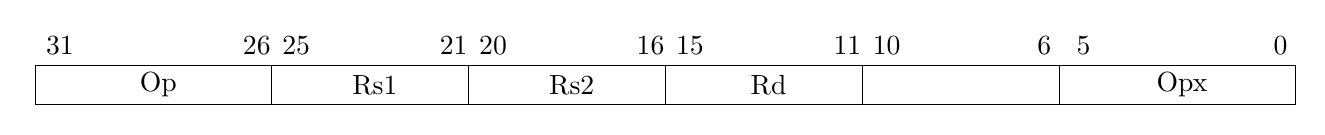
\begin{tikzpicture}[x=0.5cm, y=0.5cm]
                                \node at (0.5, 0.5) {~31~};
                                \node at (5.5, 0.5) {~26~};
                                \node at (6.5, 0.5) {~25~};
                                \node at (10.5, 0.5) {~21~};
                                \node at (11.5, 0.5) {~20~};
                                \node at (15.5, 0.5) {~16~};
                                \node at (16.5, 0.5) {~15~};
                                \node at (20.5, 0.5) {~11~};
                                \node at (21.5, 0.5) {~10~};
                                \node at (25.5, 0.5) {~6~};
                                \node at (26.5, 0.5) {~5~};
                                \node at (31.5, 0.5) {~0~};
                                \draw
                                (0, 0) -- (32, 0) -- (32, -1) -- (0, -1) -- cycle
                                (6, 0) -- (6, -1)
                                (11, 0) -- (11, -1)
                                (16, 0) -- (16, -1)
                                (21, 0) -- (21, -1)
                                (26, 0) -- (26, -1);
                                \node at (3, -0.5) {~Op~};
                                \node at (8.5, -0.5) {~Rs1~};
                                \node at (13.5, -0.5) {~Rs2~};
                                \node at (18.5, -0.5) {~Rd~};
                                \node at (29, -0.5) {~Opx~};
                            \end{tikzpicture}
                        \end{center}
                        For example, ~ADD R8, R6, R4~ sets the value of ~R8~ to be the sum of ~R6~ and ~R4~.
                    \item \textbf{register-immediate} \hfill one source and one destination register, immediate operand (e.g. adding)
                        \begin{center}
                            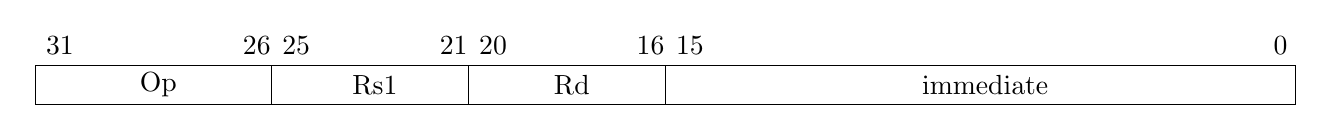
\begin{tikzpicture}[x=0.5cm, y=0.5cm]
                                \node at (0.5, 0.5) {~31~};
                                \node at (5.5, 0.5) {~26~};
                                \node at (6.5, 0.5) {~25~};
                                \node at (10.5, 0.5) {~21~};
                                \node at (11.5, 0.5) {~20~};
                                \node at (15.5, 0.5) {~16~};
                                \node at (16.5, 0.5) {~15~};
                                \node at (31.5, 0.5) {~0~};
                                \draw
                                (0, 0) -- (32, 0) -- (32, -1) -- (0, -1) -- cycle
                                (6, 0) -- (6, -1)
                                (11, 0) -- (11, -1)
                                (16, 0) -- (16, -1);
                                \node at (3, -0.5) {~Op~};
                                \node at (8.5, -0.5) {~Rs1~};
                                \node at (13.5, -0.5) {~Rd~};
                                \node at (24, -0.5) {~immediate~};
                            \end{tikzpicture}
                        \end{center}
                        Examples of this include;
                        \begin{itemize}
                            \itemsep0em
                            \item ~LW R2, 100(R3)~ \hfill ~R2 <- Memory[R3+100]~
                                \subitem source register is to be added to an immediate constant, could be useful for accessing fields of a struct (field offset is the constant) by using the base of the object
                            \item ~SW R5, 100(R6)~ \hfill ~Memory[R6+100] <- R5~
                                \subitem same as above, but for storing
                            \item ~ADDI R4, R5, 50~ \hfill ~R4 <- R5 + signExtend(50)~
                                \subitem note the sign extend; since we have a 16-bit immediate value, if it's a negative number, it needs to be padded to 32-bit
                        \end{itemize}
                    \item \textbf{branch}
                        \begin{center}
                            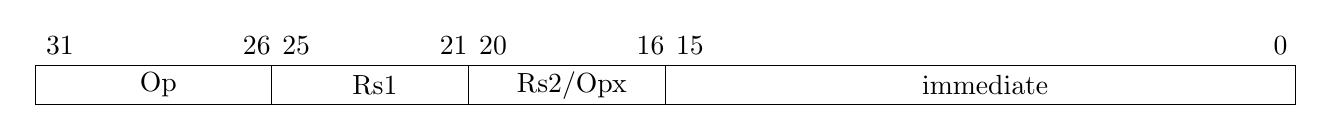
\begin{tikzpicture}[x=0.5cm, y=0.5cm]
                                \node at (0.5, 0.5) {~31~};
                                \node at (5.5, 0.5) {~26~};
                                \node at (6.5, 0.5) {~25~};
                                \node at (10.5, 0.5) {~21~};
                                \node at (11.5, 0.5) {~20~};
                                \node at (15.5, 0.5) {~16~};
                                \node at (16.5, 0.5) {~15~};
                                \node at (31.5, 0.5) {~0~};
                                \draw
                                (0, 0) -- (32, 0) -- (32, -1) -- (0, -1) -- cycle
                                (6, 0) -- (6, -1)
                                (11, 0) -- (11, -1)
                                (16, 0) -- (16, -1);
                                \node at (3, -0.5) {~Op~};
                                \node at (8.5, -0.5) {~Rs1~};
                                \node at (13.5, -0.5) {~Rs2/Opx~};
                                \node at (24, -0.5) {~immediate~};
                            \end{tikzpicture}
                        \end{center}
                        Two registers, for example if the contents are equal, then branch.
                        One challenge is that the address would have to fit in the immediate field, therefore it's not an \textbf{absolute} address, but one that's \textbf{relative} to the current program counter.
                        Note that it's multiplied by 4, as it's a fixed size.
                        For example, ~BEQ R5, R7, 25~; if ~R5 = R7~, then update ~PC <- PC + 4 + 25*4~, otherwise ~PC <- PC + 4~ (we update it regardless).
                    \item \textbf{jump / call}
                        \begin{center}
                            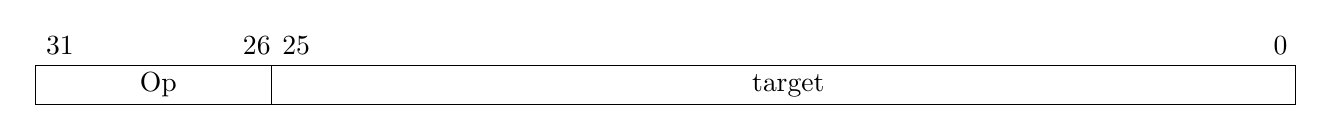
\begin{tikzpicture}[x=0.5cm, y=0.5cm]
                                \node at (0.5, 0.5) {~31~};
                                \node at (5.5, 0.5) {~26~};
                                \node at (6.5, 0.5) {~25~};
                                \node at (31.5, 0.5) {~0~};
                                \draw
                                (0, 0) -- (32, 0) -- (32, -1) -- (0, -1) -- cycle
                                (6, 0) -- (6, -1);
                                \node at (3, -0.5) {~Op~};
                                \node at (19, -0.5) {~target~};
                            \end{tikzpicture}
                        \end{center}
                        Unconditional branch, allowing for a jump to anywhere in the full address space of the machine.
                \end{itemize}
                The top bits are occupied by the opcode.
                Register specifier fields also occupy fixed positions in the instruction allowing immediate access to the registers before the instruction finishes decoding.
                In MIPS, we can have up to 32 registers in the machine as the width of the register specifier fields is 5 ($2^5 = 32$).
                The largest signed immediate operand is determined by the width of the immediate field, similarly the range of addresses of a conditional jump is the same (albeit scaled by 4).
                A general machine would execute this in a loop (the slides contain a diagram of this with the components);
                \begin{lstlisting}
                    Instr = Mem[PC]; PC += 4;
                    rs1 = Reg[Instr.rs1];
                    rs2 = Reg[Instr.rs2];
                    imm = signExtend(Instr.imm);
                    Operand1 = if (Instr.op == BRANCH) then PC else rs1
                    Operand2 = if (immediateOperand(Instr.op)) then imm else rs2
                    res = ALU(Instr.op, Operand1, Operand2)
                    switch (Instr.op) {
                      case BRANCH:
                        if (rs1 == 0) then PC = PC + imm*4; continue;
                      case STORE:
                        Mem[res] = rs1; continue
                      case LOAD:
                        Imd = Mem[res]
                    }
                    Reg[Instr.rd] = if (Instr.op == LOAD) then Imd else res
                \end{lstlisting}
                The 5 steps of the MIPS datapath are as follows - the pipelined design introduces pipeline buffers between each stage;
                \begin{enumerate}[1.]
                    \itemsep0em
                    \item instruction fetch
                    \item instruction decode, register fetch
                    \item execute, address calculation
                    \item memory access
                    \item write back
                \end{enumerate}
                The pipeline buffers allow the result of a stage to be latched in the buffer, to be used in the next clock cycle.
                This allows each instruction to progressively move down the pipeline on each successive clock tick.
                Without pipelining, the entire pipeline would operate on one clock cycle, however the number of gates along the path would determine the clock cycle time / rate - a non-pipelined processor would run slowly as there is a long path.
                In a pipelined design, the cycle time is determined by the slowest of the stages, but the length of each stage is controlled to allow for the highest possible rate.
                \medskip

                In addition to this, there is also a decode which controls what is being done (which sources to read from, for example a branch would use PC rather than a register).
                The control signals configure the multiplexers (MUX), ALU, and read / write to memory.
                The signal is carried with the corresponding instruction along the pipeline.
                \medskip

                Initially the pipeline is empty.
                With each successive cycle after the first, more of the pipeline will be used, with a new instruction being fetched at each cycle, and the preceding instruction being passed to the next pipeline stage.
                \medskip

                Pipeline doesn't make each individual instruction complete quicker; it doesn't help the \textbf{latency} of an instruction, but rather the \textbf{throughput} of the entire workload.
                The pipelining doesn't add much cost as we're using the same hardware, other than latches which add some transistor count and energy consumption.
                Adding more stages to a pipeline could lead to the clock rate being dominated by the time time the signal is spent in the latches.
                \medskip

                However, there are a number of hazards to pipelining;
                \begin{itemize}
                    \itemsep0em
                    \item \textbf{structural hazards} - particular hardware units may not be able to be used by two different pipeline stages in the same cycle
                        \smallskip

                        The \textit{PS3} was based on a highly parallel multi-core processor chip.
                        The processor had a conventional unit to run the Linux OS, but also 16 parallel accelerator units (fast but simple units, no cache, just a block of SRAM for instructions and data).
                        In cycle 4, for the first instruction, it would be accessing memory, however in the same cycle, a later instruction would be trying to fetch the instruction from the \textbf{same} memory.
                        A structural hazard occurs on simultaneous access; leading to load instructions causing an instruction fetch to stall.
                        This causes a stall (delays the instruction until the next cycle), which introduces pipeline bubbles - a missed opportunity for an instruction to be processed; once a fetch is missed, subsequent steps can't do anything in next cycles.
                        This was solved with a prefetch buffer, where a block of instructions was fetched at once.
                        Instructions were reorganised at compile time.
                    \item \textbf{data hazards} - an instruction depends on the result of an incomplete (still in pipeline) instruction (causes bubbles / stalls, can be overcome with forwarding)
                        \smallskip

                        Consider the following example;
                        \begin{lstlisting}
                            ADD R1,R2,R3
                            SUB R4,R1,R3
                            AND R6,R1,R7
                            OR R8,R1,R9
                            XOR R10,R1,R11
                        \end{lstlisting}
                        After the instruction is fetched in cycle one (for the ~ADD~), ~R2~ and ~R3~ are read in in cycle 2, available in cycle 4, but only written back in cycle 5.
                        For the ~SUB~ and ~AND~ instructions, the data would need to be sent back in time in the current idea of the pipeline, which obviously isn't feasible.
                        ~XOR~ is possible, as the register read is in cycle 6.
                        For ~OR~, this is fine \textbf{if} the register write happens in the first half of the clock cycle, and the register read happens in the second half.
                        \medskip

                        The previous assumption is that the value had to be written to the register before it could be used; however, at the end of cycle 3 the result of the ~ADD~ instruction is present in the latch after the execution stage, and could be fed directly into the ALU (same for the next instruction, but rather from the latch after the memory stage).
                        The value needs to be delayed by one clock cycle, before forwarding. % why?
                        \medskip

                        The changes to the hardware to support this are as follows (see lecture slides for diagrams);
                        \begin{itemize}
                            \itemsep0em
                            \item add forwarding / bypass paths (to the MUX, mentioned next)
                                \begin{itemize}
                                    \itemsep0em
                                    \item result of the ALU from previous cycle (latch)
                                    \item the latch after memory, for forwarding the value to the next instruction but one
                                    \item final wire takes value from memory
                                \end{itemize}
                            \item expand multiplexers before ALU to select where the operands should come from (choose one of the bypass wires if forwarding is needed)
                            \item decode needs to control bigger multiplexers to select values from bypass paths for forwarding; decode will now need to track which registers are going to be updated by incomplete instructions (the decode stage knows where the operands are going to come from, as well as what operands are still in-flight)
                        \end{itemize}
                        Data hazards can still exist even with forwarding, for example with loads, as the memory access comes later in the pipeline;
                        \begin{lstlisting}
                            LW R1,0(R2)
                            SUB R4,R1,R6
                            AND R6,R1,R7
                            OR R8,R1,R9
                        \end{lstlisting}
                        Recall that arithmetic may be involved to access memory, hence the stage has to come later.
                        For the value that is required in cycle 4 (execution of ~SUB~), the value is only available at the end of the cycle.
                        There is nothing that can be done here, leading to a bubble (also known as a load-use stall).
                        Stalls will also need to be implemented to support this.
                        \medskip

                        Software scheduling can be performed to avoid load hazards (recall that bubbles are missed opportunities for execution).
                        Consider the following code;
                        \begin{lstlisting}
                            a = b + c
                            d = e - f
                        \end{lstlisting}
                        Slow code, without the optimisation takes 10 cycles, with 2 stalls;
                        \begin{lstlisting}
                            LW    Rb,b
                            LW    Rc,c
                            STALL
                            ADD   Ra,Rb,Rc
                            SW    a,Ra
                            LW    Re,e
                            LW    Rf,f
                            STALL
                            SUB   Rd,Re,Rf
                            SW    d,Rd
                        \end{lstlisting}
                        However, the faster code swaps the order of execution by moving ~LW Re,e~ in place of the first stall and ~SW a,Ra~ in place of the second stall.
                        This takes 8 cycles and has no stalls;
                        \begin{lstlisting}
                            LW    Rb,b
                            LW    Rc,c
                            LW    Re,e
                            ADD   Ra,Rb,Rc
                            LW    Rf,f
                            SW    a,Ra
                            SUB   Rd,Re,Rf
                            SW    d,Rd
                        \end{lstlisting}
                    \item \textbf{control hazards} - we assume that we already know the next instruction to fetch, however this may not be the case as we haven't decoded the previous instruction yet (may be a jump / branch)
                        \smallskip

                        Consider the following example, where we may risk stalling for three cycles;
                        \begin{lstlisting}
                            BEQ R1,R3,36
                            AND R2,R3,R5
                            OR R6,R1,R7
                            ADD R8,R1,R9
                            XOR R10,R1,R11 # instruction 36
                        \end{lstlisting}
                        After discovering the branch outcome at cycle 3, we may suffer a bad stall.
                        This can be overcome by adding early branch determination.
                        Add an adder to add the current PC to the immediate operand (in decode stage), add check with with register file, and if it passes we can use the computed next PC value
                        All the logic for determining the branch outcome is moved as early as possible in the pipeline.
                        This still introduces a delay for one cycle, as we have to fetch the next instruction regardless (while we're computing whether we should branch or not).
                        If the branch is taken, the memory access and write back stages are blocked.
                \end{itemize}
                Simultaneous multi-threading can eliminate hazards.
                Without stalls, an instruction could be finished each cycle.
                Two program counters are maintained and the processing alternates between the two counters.
                Each thread has its own program counter and own registers, thus eliminating issues with data hazards (can still occur with memory).
                \medskip

                A simple pipeline with 5 stages can run at 5 - 9 GHz, limited by the \textbf{critical} path (slowest pipeline stage).
                The main tradeoff is to do more per cycle or to increase the clock rate.
\end{document}